% Standalone, editable source of the MDP schematic.
%   pdflatex fig_mdp_schematic_standalone.tex      -> PDF (vector)
%   pdf2svg  fig_mdp_schematic_standalone.pdf fig_mdp_schematic.svg   -> editable in Inkscape/Illustrator/Figma
% The manuscript includes the PDF with \includegraphics.
\documentclass[tikz, border=4pt]{standalone}
\usepackage[T1]{fontenc}
\usepackage{mathptmx}  % Times text and math, matching the IEEEtran body
\usepackage{amsmath}
\usetikzlibrary{arrows.meta, positioning, calc, fit, backgrounds}

\begin{document}
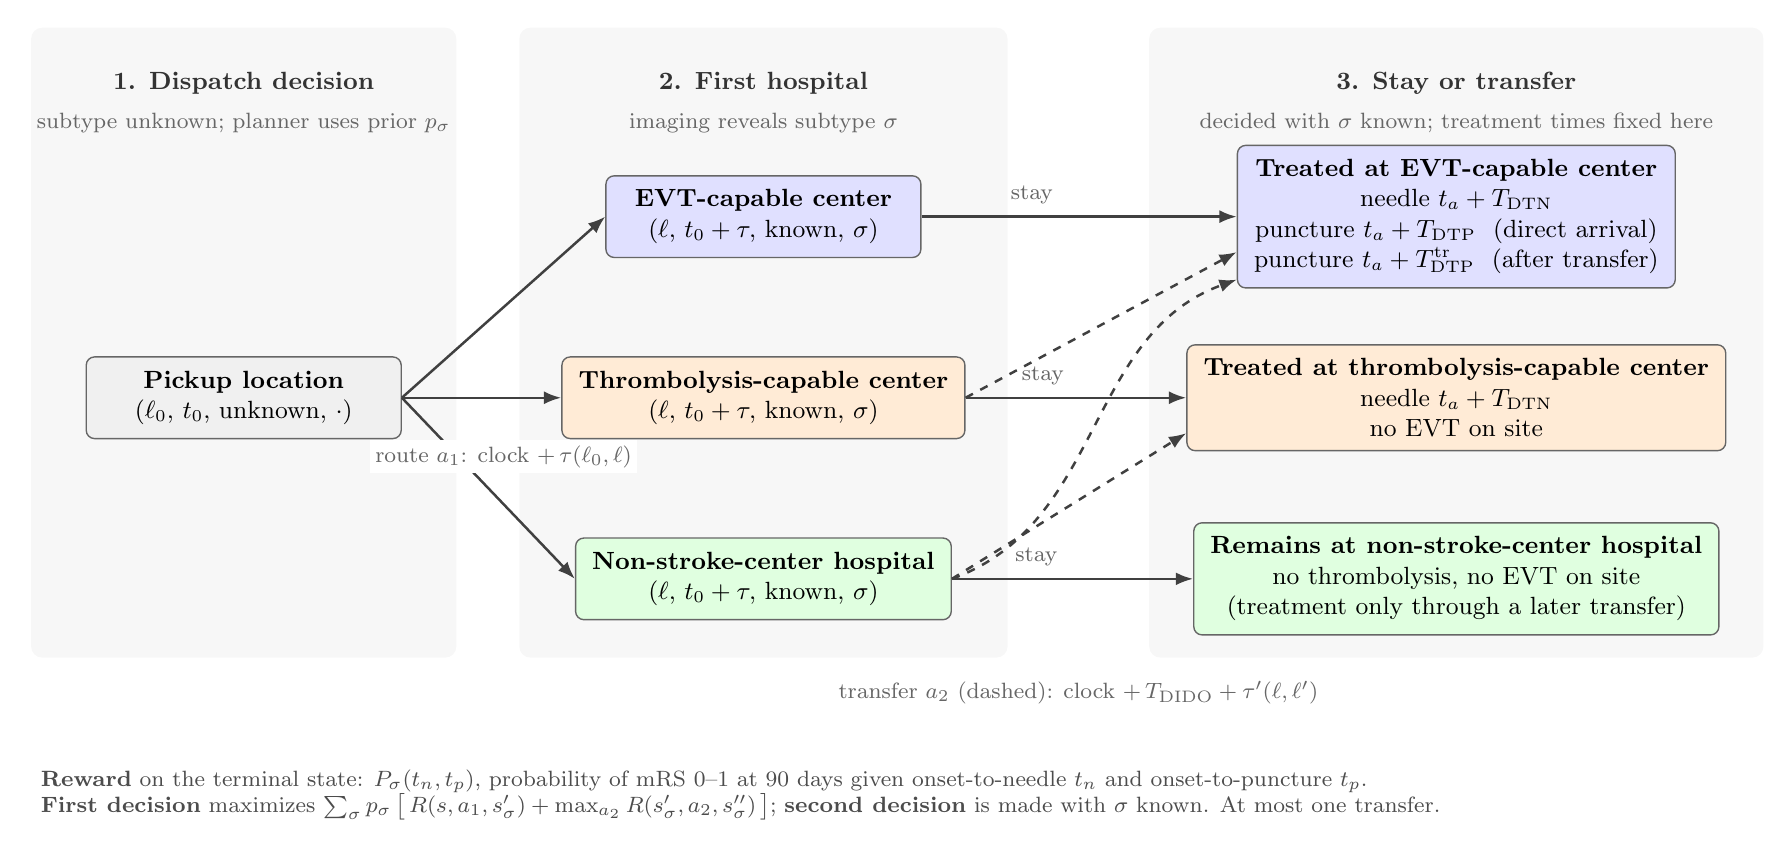
\begin{tikzpicture}[
  font=\small,
  node distance=6mm,
  box/.style={draw=black!60, line width=0.5pt, rounded corners=3pt, align=center, inner xsep=6pt, inner ysep=5pt, minimum width=40mm},
  field/.style={box, fill=black!6},
  evt/.style={box, fill=blue!12},
  psc/.style={box, fill=orange!16},
  nsc/.style={box, fill=green!12},
  route/.style={-{Latex[length=2.2mm]}, line width=0.9pt, black!75},
  xfer/.style={-{Latex[length=2.2mm]}, line width=0.9pt, black!75, dashed},
  stay/.style={-{Latex[length=2.2mm]}, line width=0.9pt, black!75},
  head/.style={font=\small\bfseries, text=black!80, align=center},
  sub/.style={font=\footnotesize, text=black!60, align=center},
  lane/.style={fill=black!3, rounded corners=4pt, draw=none}]

% ---------- column headers
\node[head] (h1) at (0,4.0)    {1. Dispatch decision};
\node[sub, below=0mm of h1]    {subtype unknown; planner uses prior $p_\sigma$};
\node[head] (h2) at (6.6,4.0)  {2. First hospital};
\node[sub, below=0mm of h2]    {imaging reveals subtype $\sigma$};
\node[head] (h3) at (15.4,4.0) {3. Stay or transfer};
\node[sub, below=0mm of h3]    {decided with $\sigma$ known; treatment times fixed here};

% ---------- column 1
\node[field] (F) at (0,0) {\textbf{Pickup location}\\$(\ell_0,\,t_0,\,\text{unknown},\,\cdot)$};

% ---------- column 2
\node[evt] (E1) at (6.6, 2.3)  {\textbf{EVT-capable center}\\$(\ell,\,t_0+\tau,\,\text{known},\,\sigma)$};
\node[psc] (P1) at (6.6, 0)    {\textbf{Thrombolysis-capable center}\\$(\ell,\,t_0+\tau,\,\text{known},\,\sigma)$};
\node[nsc] (N1) at (6.6,-2.3)  {\textbf{Non-stroke-center hospital}\\$(\ell,\,t_0+\tau,\,\text{known},\,\sigma)$};

% ---------- column 3 (terminal states with treatment timing)
\node[evt] (E2) at (15.4, 2.3) {\textbf{Treated at EVT-capable center}\\needle $t_a + T_{\mathrm{DTN}}$\\puncture $t_a + T_{\mathrm{DTP}}$ \ (direct arrival)\\puncture $t_a + T^{\mathrm{tr}}_{\mathrm{DTP}}$ \ (after transfer)};
\node[psc] (P2) at (15.4, 0)   {\textbf{Treated at thrombolysis-capable center}\\needle $t_a + T_{\mathrm{DTN}}$\\no EVT on site};
\node[nsc] (N2) at (15.4,-2.3) {\textbf{Remains at non-stroke-center hospital}\\no thrombolysis, no EVT on site\\(treatment only through a later transfer)};

% ---------- arrows: routing (column 1 -> 2), one shared label
\draw[route] (F.east) -- (E1.west);
\draw[route] (F.east) -- (P1.west);
\draw[route] (F.east) -- (N1.west);
\node[sub, fill=white, inner sep=2pt] at (3.3,-0.75) {route $a_1$: clock $+\,\tau(\ell_0,\ell)$};

% ---------- arrows: stay (solid) and transfer (dashed), column 2 -> 3
\draw[stay] (E1.east) -- node[sub, above=1pt, pos=0.35] {stay} (E2.west);
\draw[stay] (P1.east) -- node[sub, above=1pt, pos=0.35] {stay} (P2.west);
\draw[stay] (N1.east) -- node[sub, above=1pt, pos=0.35] {stay} (N2.west);
\draw[xfer] (P1.east) -- ($(E2.west)+(0,-0.45)$);
\draw[xfer] (N1.east) -- ($(P2.west)+(0,-0.45)$);
\draw[xfer] (N1.east) to[out=20, in=200] ($(E2.west)+(0,-0.8)$);
\node[sub, fill=white, inner sep=2pt, align=left] at (10.6,-3.75) {transfer $a_2$ (dashed): clock $+\,T_{\mathrm{DIDO}} + \tau'(\ell,\ell')$};

% ---------- imaging line between columns 2 and 3 is implied by the headers; reward note at the bottom
\node[sub, align=left, anchor=north west, text=black!70] at (-2.7,-4.6)
  {\textbf{Reward} on the terminal state: $P_\sigma(t_n, t_p)$, probability of mRS 0--1 at 90 days given onset-to-needle $t_n$ and onset-to-puncture $t_p$.\\
   \textbf{First decision} maximizes $\sum_\sigma p_\sigma\,\big[\,R(s,a_1,s'_\sigma) + \max_{a_2} R(s'_\sigma,a_2,s''_\sigma)\,\big]$; \textbf{second decision} is made with $\sigma$ known. At most one transfer.};

% ---------- lane backgrounds (explicit, identical height)
\begin{scope}[on background layer]
  \fill[lane] (-2.7,-3.3) rectangle (2.7,4.7);
  \fill[lane] (3.5,-3.3) rectangle (9.7,4.7);
  \fill[lane] (11.5,-3.3) rectangle (19.3,4.7);
\end{scope}
\end{tikzpicture}
\end{document}
